% !TeX root = ../main.tex
% Add the above to each chapter to make compiling the PDF easier in some editors.

\chapter{Background}\label{chapter:background}
\section{Manipulation and Grasping}
% !TeX root = ../main.tex
% Add the above to each chapter to make compiling the PDF easier in some editors.

\section{Reinforcement Learning}

The simplest examples of learning come from our own life; we learn to walk, speak the language, or to cook. All those activities span our entire life, it influences who we are and the decisions we take in life. We know that living animals such as mammals learn from their social and asocial interactions with the environment.
We know that living animals such as mammals learn from their social and asocial interactions with the environment \cite{AnimalInt11}. 
Although we have not yet developed a full-scale theory of animal learning, we have developed computational objectives for machines to learn \cite{Sutton2018}. 
This computational approach can be categorized as Supervised, Unsupervised or Reinforcement Learning. This computational approach falls into three categories as Supervised, Unsupervised, or Reinforcement Learning.

In this chapter, we will consider the Reinforcement Learning objectives and problem formulation.
Reinforcement Learning provides a systematic approach to maximize the reward by linking observations to actions. A reinforcement learning agent creates its data by interacting with the environment. Therefore, it is fundamentally different from supervised and unsupervised learning, where the data is already provided \cite{Sutton2018}. 
Another important difference is the inherent goal-oriented approach. Reinforcement learning agent maximizes the rewards for its inherent general goal. Other machine learning approaches lack this goal \cite{Sutton2018}.
For instance, supervised learned software recognizing faces can be used for security reasons to detect criminals or can be easily used to unlock phones. However, a reinforcement learning agent trained to drive a car autonomously can only drive a car. In a sense, reinforcement learning provides us end-to-end learning.

A core feature of reinforcement learning is that it acts on uncertain environments and, in return, receives the observation and reward. Fundamentally, a learning agent collects this experience and tunes its action to increase the expected reward. The expected reward term refers to the end of the horizon. For example, a chess-playing agent can choose to sacrifice the queen in the next move for a checkmate in the move after. In this case, the reward would decrease when the agent loses a queen, but the goal of the agent will be satisfied by terminating the game. For a well-defined reinforcement learning system, we can speak of four main components: Policy to decide the actions, a reward to maximize the expected reward in the horizon, and a model of the environment, telling which directions the chess pieces can move. The components of reinforcement learning are formulated based on Markov Decision Process. In the MDP chapter, we will detailly explain RL components. In the next chapters first Markov Chains, the simple version of MDP, then MDP, the slightly advanced version of Markov Chains, will be explained by some simple modifications \cite{PerezMIT}.

\subsection{Markov Chain}

The weak law of large numbers has a tremendous significance on stochastic modeling. This law states that the average of a large number of experimentations converges to the real value of the probability of a particular task. As an example, if one tosses infinite amounts of the coin, the average number of heads should converge to 0.5 \cite{Gagniuc2017}. 
Bernoulli’s weak law of large numbers only covers independent events. Markov proved that Bernoulli’s law also holds on dependent cases \cite{Gagniuc2017}. 
As the law of large numbers suggests, if one conducts a large number of iterations on this problem, one can deduce the transition matrix. This matrix proves to be the only information one needs to compute the next state.
This characteristic defines the famous Markov property; the current state captures all the necessary information one needs to predict the next state. If we extrapolate this example to slightly complex systems, for example, weather forecast, we just need today’s weather report to predict tomorrow’s forecast, assuming that we know the transition matrix. Naturally, one can formulate other events with Markov Chain lawnmower, and random walk are the straightforward ones in the literature\cite{Gagniuc2017}.

It is also possible to attach rewards to Markov Chain’s formulation. In figure \ref{fig: markov_chain}, the transition between states is represented with the arcs. And each transition has a probability similar to the transition matrix; we defined before. Each state has an immediate reward and a value function. The immediate reward is received directly when the actor moves to that state. The value of a state represents how likely the future actor will end up collecting high rewards. 

\begin{figure}[htbp]
    \centering
    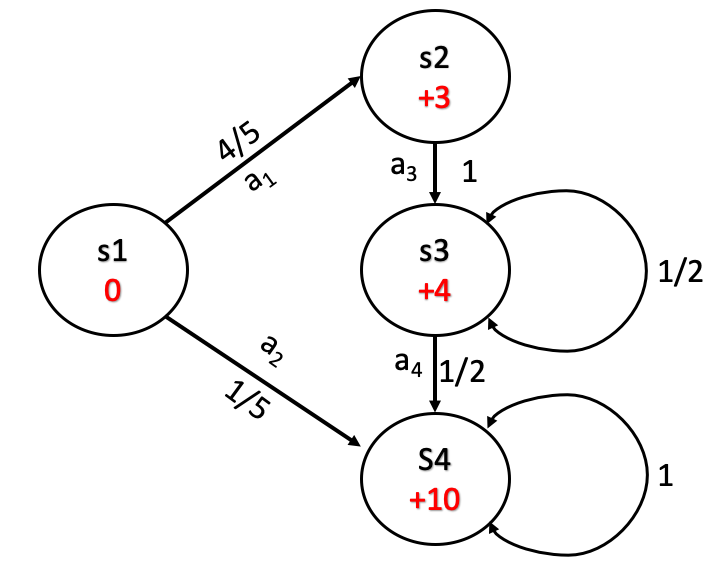
\includegraphics[width=0.5\textwidth]{figures/markovchain}
    \caption{Markov chain with transition probabilties and rewards}
    \label{fig: markov_chain}
\end{figure}

The value of a state will be later significant to solve Reinforcement Learning problems through Value Iteration methods. They are one of the essential algorithms that led to the initial success of Reinforcement Learning research.

    \subsection{Markov Decision Process}\label{section:markov}

Markov decision process is a slightly advanced version of the Markov Chain. It includes action on top of the Markov Chain. Reinforcement learning problems are formalized as a Markov Decision Process rather than Markov Chain because RL agents are free to choose from different actions.

MDPs first came into play as part of optimal control problem by Bellman \cite{Bellman1958}. Bellman applied dynamic programming methods to solve the MDP problem optimally. However, this methodology was not scalable to larger problems stem from the curse of dimensionality problem \cite{Sutton}.

The fundamental elements of MDP are as follows:
\begin{itemize}
    \item Agent:  The actor takes action on the environment to learn.
    \item Environment: The agent interacts with the Environment(Plant).
    \item Rewards: Environment returns rewards based on the interaction made by the actor.
    \item State: View of the environment from the eyes of the actor. 
\end{itemize}

\begin{figure}[htbp]
    \centering
    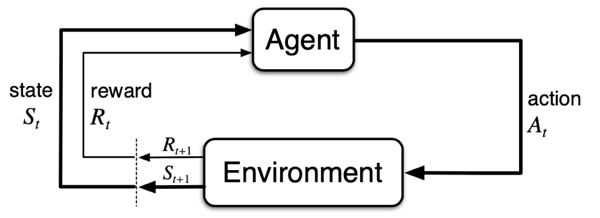
\includegraphics[width=0.8\textwidth]{figures/mdp}
    \caption{MDP structure}
    \label{fig: mdp}
\end{figure}

The process of action follows; the agent acts on the environment at time t and environment return the reward and state of the action at time \(t+1\). Based on the state of the environment at the \(t+1\) agent makes another action \(A_{t+1}\), which results in \(R_{t+2}\) and \(S_{t+2}\).

In every MDP system, agents should be reachable to every state through a sequence of actions. The transition between states is of great value for the MDP framework.
One can compute the transition probability in MDP, given the inner dynamics of the environment \cite{Sutton2018}. The below equation defines the internal dynamics probability. It tells, how probable it is to end up in state s’ with reward r by taking action a in state s. 

\begin{equation}
    p(s',r | s,a) = Pr\{S_t = s', R_t = r | S_{t-1} = d, A_{t-1} = a\}
\end{equation}

One can calculate the transition probability function from the inner dynamics’ probability function.

\begin{equation}
    p(s'|s,a) = Pr\{S_t=s'| S_{t-1}=s, A_{t-1}=a\} = \sum_{r \in R}p(s',r|s,a)
\end{equation}

Next chapter, we will dive into the definition of the reward and value function. Based on those concepts we will build the logic on how to solve MDPs optimally
    \subsection{Reward and Value function}
% \todo{Ilk paragraf} 

As defined in the Markov Chain section, rewards and value functions are the essence of value iteration algorithms. In this section, we will describe the objective of the RL problem formally. As we mentioned in previous chapters, we want the increase the sum of rewards we achieve at the terminal state. If we define the reward at the final state \(T\) as \(R_T\) and the reward at the initial state \(t\) is \(R_t\), the returns we receive is the sum of rewards in every state.

\begin{equation}
    G_t = R_{t+1} + R_{t+2} + R_{t+3} + ... + R_T    
\end{equation}


\(G_t\) is the notation of expected return. We will mostly use the discounted version of the expected return calculation. We introduce a discount factor \(\gamma\) to value the rewards that the agent receives now, compare to the rewards in the future. 
\begin{equation}
    G_t = R_{t+1} + \gamma^1*R_{t+2} + \gamma^2*R_{t+3} + ... + \gamma^T-1*R_T = \sum\limits_{k=0}\gamma^kR_{t+k+1}
\end{equation}

For instance, if a rational human offered to choose between 1m Euros now, versus 1m Euros in 50 years, would usually choose 1m Euros now. Therefore, our agent also weighs the rewards it receives now, over 50 steps from the current state.  In the meantime, we do not want the agent to undervalue the importance of reaching the terminal state through the highest reward sequence.  Given the below example (\ref{fig: nonoptimal}), if we introduce a discount factor of 0, the agent will always try to maximize the immediate reward and take a sequence of s1-a2-s3-a4-s4 and end up with a non-optimal greedy algorithm with \(G_t = 20 \). But with a discount factor, in this example everything between \(0< \gamma < 1\) works, would find the optimal sequence  s1-a1-s2-a3-s4 with \(G_t = 25\).

\begin{figure}[!htbp]
    \centering
    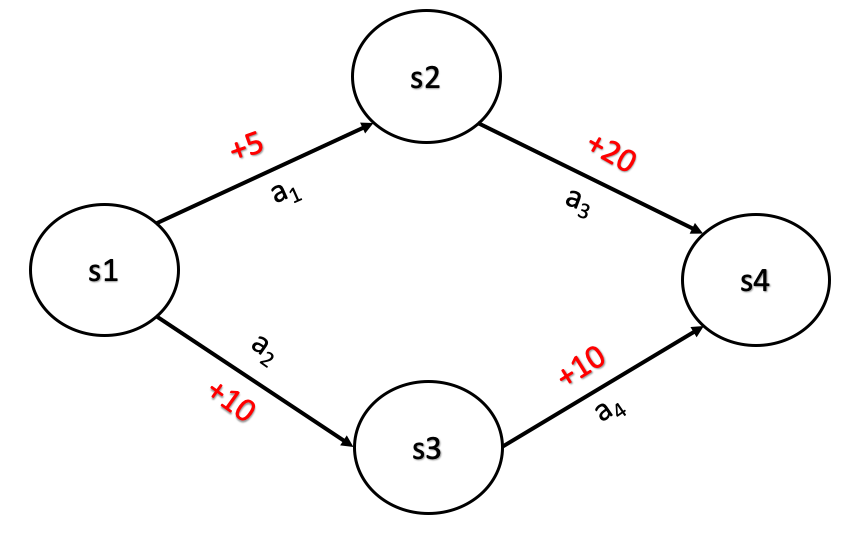
\includegraphics[width=0.6\textwidth]{figures/nonoptimal}
    \caption{Zero discount factor leads to non-optimal solution with s1-a2-s3-a4-s4. Discount factor greater than zero leads finds the optimal solution of s1-a1-s2-a3-s4 }
    \label{fig: nonoptimal}
\end{figure}

The value function is the expectation of returns, while an agent follows the policy (\(\pi\)). The policy represents the probability distribution of an agent taking action \(a\) in state \(s\). The policy is similar to the transition probability matrix in the Markov Chain section. Using policy, we can define the value function of an agent following the policy pi as below.
    \subsection{Q-Learning}

Q-learning algorithms have been the core of the RL research for almost 20 years. It combines the idea of TD learning in approximating action-value function. Through this approach, the computation converges faster than state-value approximation algorithms. Another strength of the Q-learning algorithm is its off-policy nature. The Q-learning agent can learn from the experiences of different policies. The off-policy nature makes the agent more data-efficient.

\begin{equation}
    Q(S_t, A_t) \longleftarrow Q(S_t, A_t) + \alpha [R_{t+1} + \gamma \max\limits_{a}Q(S_{t+1}, a)- Q(S_t, A_t))] 
\end{equation}

    \subsection{Value-Based Reinforcement Learning}
        \subsubsection{Q-network}
        \subsubsection{Extension of Q-networks}
        \subsubsection{Branch Dueeling Q-networks}
    \subsection{Policy-Based Reinforcement Learning}
        \subsubsection{Entropy-Based Approach}
        \subsubsection{Soft Actor Critic}
    \subsection{Off-Policy RL}
    \subsection{On-Policy RL}
\section{Neural Networks}


% !TeX root = ../main.tex
% Add the above to each chapter to make compiling the PDF easier in some editors.

\section{Curriculum Learning}


One can gradually increase the level of the difficulty of a specific task to be learned to guide the training process and speed up the convergence time. Based on phycological studies, humans learn faster when they subject to the information in the form of a unique curriculum. That is because we are subjected to curriculum learning since they were toddlers. 


% !TeX root = ../main.tex
% Add the above to each chapter to make compiling the PDF easier in some editors.

\section{Simulator Choice}

    \subsection{Mujoco}
    \subsection{Gazebo}
    \subsection{PyBullet}
\section{State of Art}
    \subsection{Dexnet}
    \subsection{DQL Google}
